\section{Performance, Results, and Discussion}\label{sec:7}

This chapter presents TraceAdvisor's offline evaluation results, focusing on the tradeoff between under-provisioning and excess resource allocation. Preliminary studies on three Azure traces examine historical baselines, while Google ClusterData 2019 \cite{ref7} serves as the primary evaluation dataset and Alibaba GPU 2020 \cite{ref19} provides a second recurring-workload evaluation. Validation results are used to describe policy and model selection, while final-test results assess the selected approaches. The chapter also compares findings across the two datasets and discusses evaluation limitations.

\subsection{Preliminary Baseline Studies on Azure Traces}\label{sec:7.1}

Before the TraceAdvisor design was fixed, baseline sizing experiments were run on three Azure traces: Resource Central, Splitwise, and ModServe (Section~\ref{sec:3.3.3}). None describes recurring jobs with a per-job request and per-job CPU and memory usage, so they establish the tradeoff that motivated the design rather than results for the recommendation policies.

The Resource Central study uses a sample of 100,000 CPU readings from 100,000 virtual machines. The VM-level analysis shows a mean difference of 6.977 percentage points and a median difference of 2.295 percentage points between P95 and mean CPU usage. Mean-based and P95-based CPU bucket assignments agree for 87.11\% of the sampled virtual machines. However, this agreement reflects consistency between the two classification methods rather than predictive accuracy on unseen data. An important limitation is that each sampled VM contains only one reading. The reported P95 is derived from the reading's maximum CPU field, while the mean is derived from its average CPU field. Consequently, these measurements do not represent long-term historical CPU percentiles for individual VMs.

The Splitwise study evaluates fixed capacities derived from a training period against later token-demand windows. For code requests, a capacity at the training mean was exceeded in 33.3\% of the 24 test windows, while P95 and P99 capacities were exceeded in 4.2\% and 0\% of windows at average utilizations of 0.37 and 0.24, compared with 0.82 for the mean.

The ModServe study compares fixed and reactive capacity policies for image and text serving, with demand converted into capacity units per window. Over 720 test windows, the fixed policy provisioned 19 units against an average requirement of 5.4 and was safe in 95.3\% of windows, while the reactive policy provisioned close to the average requirement but was safe in only 71.5\% of windows.

All three studies show the same pattern: sizing near average demand is efficient but frequently short, while sizing at a high percentile is safe but wasteful. They do not evaluate memory, recurrence-based prediction, or the ML and Hybrid policies.

\subsection{Google ClusterData 2019 Results}\label{sec:7.2}

The Google experiment uses a Kaggle sample of ClusterData 2019 \cite{ref7}. Resource recommendations are evaluated against the next workload occurrence's peak CPU and memory usage, expressed in Google's normalized resource units. The saved evaluation includes 329 validation occurrences and 259 final-test occurrences with valid CPU and memory targets. These results reflect occurrence-level evaluations of the sampled dataset rather than the complete Google trace. Additional evaluation limitations are discussed in Section~\ref{sec:7.5}.

Violation rate, waste, shortfall, and bounded utilization are defined in Section~\ref{sec:4.3}; an any-resource violation occurs when either CPU or memory demand exceeds its recommendation. These metrics evaluate offline resource-sizing performance and do not directly measure application latency, scheduling efficiency, or actual financial savings.

\subsubsection{Baseline Recommendation Results}\label{sec:7.2.1}

The baseline comparison includes Request, Mean, P90, P95, and P99. Request uses the originally declared CPU and memory resource requests, while the remaining policies calculate recommendations using statistics from previously completed workload occurrences. When sufficient historical data is unavailable, these policies fall back to the original resource requests.

During validation, P99 with \texttt{min\_runs\ =\ 1} was selected because it achieved the lowest any-resource violation rate among the evaluated baseline candidates. This selection was based on validation performance and is separate from the final-test results presented in Table~\ref{tab:7.1}.

\begin{table*}[!t]
\centering
\footnotesize
\caption{Google final-test baseline results (violation rates in \%, average waste in normalized units)}\label{tab:7.1}
\begin{tabular}{>{\raggedright\arraybackslash}p{0.109\linewidth}>{\raggedright\arraybackslash}p{0.158\linewidth}>{\raggedright\arraybackslash}p{0.158\linewidth}>{\raggedright\arraybackslash}p{0.206\linewidth}>{\raggedright\arraybackslash}p{0.109\linewidth}>{\raggedright\arraybackslash}p{0.109\linewidth}}
\hline
\textbf{Policy} & \textbf{CPU violation (\%)} & \textbf{Memory violation (\%)} & \textbf{Any-resource violation (\%)} & \textbf{CPU waste} & \textbf{Memory waste} \\ \hline
Request & 50.58 & 34.24 & 54.47 & 0.498 & 0.176 \\
Mean & 28.57 & 33.59 & 38.22 & 1.226 & 0.235 \\
P90 & 18.15 & 16.60 & 22.78 & 3.847 & 0.744 \\
P95 & 13.13 & 13.13 & 17.37 & 7.616 & 1.541 \\
P99 & 9.27 & 11.97 & 14.67 & 17.483 & 2.994 \\
\hline
\end{tabular}
\end{table*}

The final-test evaluation includes 259 workload occurrences. The Request baseline has 257 valid observations for each violation rate, while the remaining baseline policies have 259. Missing recommendations are excluded from the calculations rather than treated as nonviolations.

Request has the highest CPU and memory violation rates, indicating that declared resource requests frequently fall below the next occurrence's observed peak usage. Mean improves reliability but still results in substantial under-provisioning. Moving from Mean to higher-percentile baselines progressively reduces violation rates while increasing average resource waste. P99 achieves the lowest CPU and memory violation rates among the historical baselines, although its average resource waste is considerably higher than P95.

This tradeoff reflects how percentile-based recommendations are calculated. Higher percentiles account for occasional spikes in historical resource usage by recommending greater capacity, which can reduce the likelihood of under-provisioning. However, this additional capacity may remain unused when actual demand is lower. These findings illustrate the tradeoff between reliability and resource efficiency rather than identifying a single baseline that performs best across all metrics.

Fig.~\ref{fig:7.1} illustrates the validation results used for baseline selection, while Table~\ref{tab:7.1} presents the separate final-test results.

\begin{figure*}[!t]
\centering
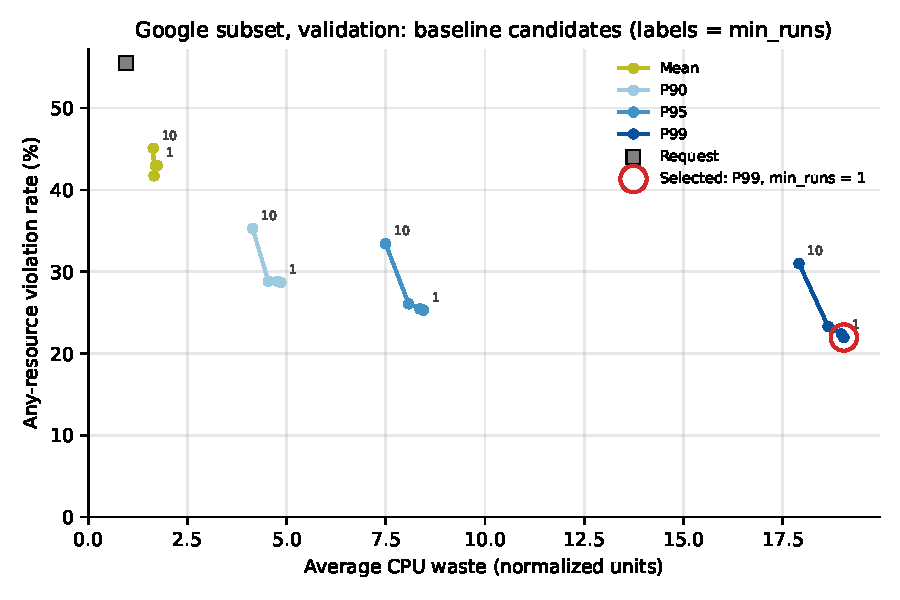
\includegraphics[width=0.92\linewidth]{figures/fig_7_1.pdf}
\caption{Google validation baseline candidates: any-resource violation rate versus average CPU waste, with \texttt{min\_runs} at the line ends and the selected P99 candidate (\texttt{min\_runs\ =\ 1}) circled}\label{fig:7.1}
\end{figure*}

\subsubsection{ML and Hybrid Recommendation Results}\label{sec:7.2.2}

Random Forest was selected independently for CPU and memory based on the lowest validation root mean squared error (RMSE) on the log1p scale among the evaluated Decision Tree, Random Forest, and XGBoost models. For CPU, Random Forest achieved a validation RMSE of 0.850, compared with 0.860 for XGBoost and 0.891 for Decision Tree. For memory, Random Forest achieved an RMSE of 0.387, compared with 0.439 for XGBoost and 0.421 for Decision Tree.

Although Random Forest achieved the lowest validation errors among the evaluated models, its predictive performance on the original resource scale was limited, with R$^{2}$ values of $-$0.005 for CPU and 0.107 for memory. These measurements reflect validation performance and should not be interpreted as final-test regression results.

Following model selection, the selected Random Forest models were retrained using eligible training and validation data before generating final-test predictions. The ML policy uses the model predictions directly, while the Hybrid policy recommends the maximum of the ML prediction and the historical P95 recommendation for each resource. When a historical P95 recommendation is unavailable, Hybrid uses the ML prediction alone. The P95 safeguard was established in advance and differs from the P99 baseline selected during validation.

\begin{table*}[!t]
\centering
\footnotesize
\caption{Google final-test comparison of ML, Hybrid, and historical baselines (paired values are CPU / memory; waste and shortfall in normalized units)}\label{tab:7.2}
\begin{tabular}{>{\raggedright\arraybackslash}p{0.072\linewidth}>{\raggedright\arraybackslash}p{0.107\linewidth}>{\raggedright\arraybackslash}p{0.107\linewidth}>{\raggedright\arraybackslash}p{0.142\linewidth}>{\raggedright\arraybackslash}p{0.130\linewidth}>{\raggedright\arraybackslash}p{0.142\linewidth}>{\raggedright\arraybackslash}p{0.130\linewidth}}
\hline
\textbf{Policy} & \textbf{CPU violation (\%)} & \textbf{Memory violation (\%)} & \textbf{Any-resource violation (\%)} & \textbf{Utilization (CPU / memory)} & \textbf{Waste (CPU / memory)} & \textbf{Shortfall (CPU / memory)} \\ \hline
P95 & 13.13 & 13.13 & 17.37 & 0.278 / 0.342 & 7.616 / 1.541 & 0.371 / 0.043 \\
P99 & 9.27 & 11.97 & 14.67 & 0.233 / 0.297 & 17.483 / 2.994 & 0.220 / 0.039 \\
ML & 30.12 & 18.92 & 32.82 & 0.431 / 0.312 & 0.424 / 0.130 & 1.065 / 0.165 \\
Hybrid & 10.81 & 7.72 & 12.36 & 0.242 / 0.190 & 7.637 / 1.546 & 0.365 / 0.042 \\
\hline
\end{tabular}
\end{table*}

All reported violation rates are based on 259 valid observations. CPU utilization is calculated using 258 observations for P95 and P99 and 259 for ML and Hybrid, while memory utilization is calculated using 259 observations for all four policies.

Hybrid achieves the lowest any-resource violation rate at 12.36\%, compared with 14.67\% for P99 and 17.37\% for P95. It also achieves the lowest memory violation rate among the evaluated policies. Compared with its P95 safeguard, Hybrid reduces violation rates with only a small increase in average resource waste. Compared with P99, Hybrid achieves both lower average waste and fewer any-resource violations. However, P99 maintains a lower CPU violation rate and lower average shortfall for both CPU and memory.

ML alone produces the lowest average CPU and memory waste, but its any-resource violation rate remains high at 32.82\%. Its average CPU and memory shortfalls are also substantially greater than those of Hybrid. These findings indicate that reducing resource waste does not necessarily result in reliable recommendations. By incorporating the historical P95 safeguard, Hybrid provides more conservative resource recommendations, although its lower bounded utilization reflects the additional capacity recommended to reduce under-provisioning. These findings are based on the saved final-test evaluation and do not establish statistical significance or generalizability across repeated experiments.

Fig.~\ref{fig:7.2} illustrates the resource-specific tradeoffs between violation rates and average waste observed during final-test evaluation, complementing the results presented in Tables~\ref{tab:7.1} and~\ref{tab:7.2}.

\begin{figure*}[!t]
\centering
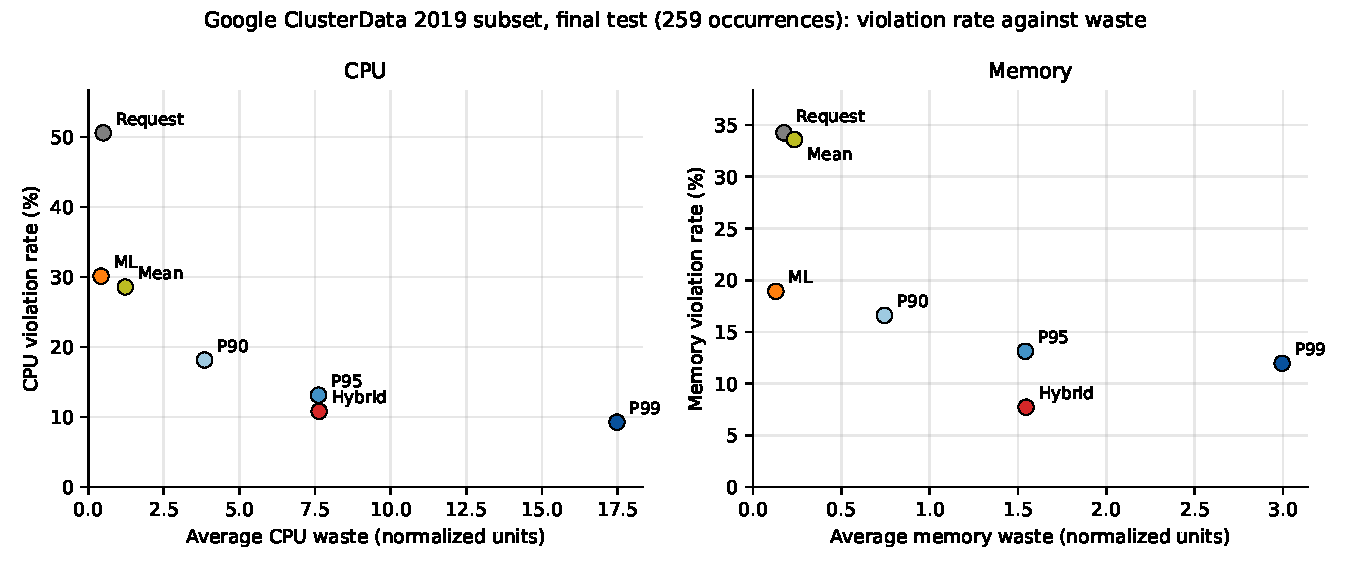
\includegraphics[width=0.92\linewidth]{figures/fig_7_2.pdf}
\caption{Google final test: CPU (left) and memory (right) violation rate versus average waste in normalized units, 259 occurrences}\label{fig:7.2}
\end{figure*}

\subsection{Alibaba GPU 2020 Results}\label{sec:7.3}

The Alibaba GPU 2020 dataset \cite{ref19} was evaluated using historical baseline policies, machine learning (ML) predictions, and Hybrid recommendations. The validation dataset contains 42,069 valid memory targets and 41,913 valid CPU targets, while the final-test dataset contains 44,053 valid memory targets and 44,045 valid CPU targets. To preserve chronological separation, next-occurrence targets are restricted to successors within the same data split. The results represent eligible completed workload roles with sufficient memory telemetry.

\subsubsection{Baseline Recommendation Results}\label{sec:7.3.1}

During validation, P99 with \texttt{min\_runs\ =\ 10} was selected using a memory-first ranking that prioritized memory violation rate, memory waste, CPU violation rate, and CPU waste, in that order. Request was included as a reference policy but was not eligible for selection. At the selected history threshold, P99 achieved a validation memory violation rate of 5.58\% and average memory waste of 8.941 GB, compared with 4.74\% and 22.255 GB for Request. Although P99 reduced average memory waste, Request achieved a lower memory violation rate during validation.

Table~\ref{tab:7.3} presents the validation and final-test results separately. All historical baseline policies shown use \texttt{min\_runs\ =\ 10} and fall back to the original resource request when sufficient historical data is unavailable.

\begin{table*}[!t]
\centering
\footnotesize
\caption{Alibaba GPU 2020 validation and final-test results (CPU is the maximum lifetime-average usage across a role's instances, in percent of one vCPU; memory waste in GB per instance)}\label{tab:7.3}
\begin{tabular}{>{\raggedright\arraybackslash}p{0.186\linewidth}>{\raggedright\arraybackslash}p{0.145\linewidth}>{\raggedright\arraybackslash}p{0.248\linewidth}>{\raggedright\arraybackslash}p{0.145\linewidth}>{\raggedright\arraybackslash}p{0.145\linewidth}}
\hline
\textbf{Split} & \textbf{Policy} & \textbf{Violation (CPU / memory, \%)} & \textbf{CPU waste} & \textbf{Memory waste (GB)} \\ \hline
Validation & Request & 15.52 / 4.74 & 430.06 & 22.255 \\
Validation & Mean & 40.84 / 39.90 & 142.56 & 6.851 \\
Validation & P90 & 12.25 / 12.40 & 235.44 & 7.803 \\
Validation & P95 & 9.00 / 8.46 & 263.08 & 8.260 \\
Validation & P99 & 6.62 / 5.58 & 294.96 & 8.941 \\
Validation & ML & 41.91 / 47.76 & 86.50 & 1.903 \\
Validation & Hybrid & 4.60 / 5.15 & 305.62 & 9.141 \\
Final test & Request & 16.71 / 3.16 & 419.97 & 22.313 \\
Final test & Mean & 41.83 / 37.02 & 138.75 & 6.451 \\
Final test & P90 & 12.41 / 9.89 & 237.57 & 7.440 \\
Final test & P95 & 9.10 / 6.04 & 266.95 & 7.895 \\
Final test & P99 & 6.45 / 3.44 & 306.44 & 8.668 \\
Final test & ML & 47.37 / 44.77 & 72.01 & 1.328 \\
Final test & Hybrid & 3.77 / 3.15 & 326.82 & 8.707 \\
\hline
\end{tabular}
\end{table*}

\subsubsection{ML and Hybrid Recommendation Results}\label{sec:7.3.2}

HistGradientBoosting was selected independently for CPU and memory based on validation RMSE among candidate models evaluated with fixed settings. The selected models achieved validation RMSE values of 412.94 in percent-of-vCPU units for CPU and 8.98 GB for memory, with R$^{2}$ values of 0.758 and 0.529, respectively. These measurements reflect validation performance used for model selection, not final-test regression performance.

Unlike the Google evaluation, which uses historical P95 as its Hybrid safeguard, Alibaba uses the validation-selected P99 baseline. For each resource, Hybrid recommends the maximum of the ML prediction and the historical P99 recommendation. Following model selection, the selected models were retrained using the combined training and validation data before generating final-test predictions.

During validation, Hybrid achieved CPU and memory violation rates of 4.60\% and 5.15\%, compared with 41.91\% and 47.76\% for ML alone. Because these results were obtained from the model-selection split, they should not be interpreted as independent test evidence. The separate final-test results in Table~\ref{tab:7.3} show that Hybrid maintains lower violation rates for both resources, while ML alone remains substantially more prone to under-provisioning.

In the final-test evaluation, Hybrid achieved a memory violation rate of 3.15\%, compared with 3.44\% for P99, 6.04\% for P95, 9.89\% for P90, and 37.02\% for Mean. Request achieved a similar memory violation rate of 3.16\%, but produced substantially greater average memory waste at 22.313 GB, compared with 8.707 GB for Hybrid and 8.668 GB for P99.

Hybrid also achieved a CPU violation rate of 3.77\%, compared with 6.45\% for P99, 16.71\% for Request, and 47.37\% for ML, at 6.7\% more average CPU waste than P99 (326.82 versus 306.44). However, Alibaba CPU targets represent the maximum lifetime-average CPU usage across instances within a workload role, rather than peak CPU demand. Therefore, these results evaluate average-usage resource sizing and do not establish protection against CPU usage peaks.

ML alone produced the lowest average memory waste at 1.328 GB, but had a substantially higher memory violation rate of 44.77\%. Hybrid also achieved a lower average memory shortfall of 0.197 GB, compared with 0.233 GB for P99 and 1.046 GB for ML.

Fig.~\ref{fig:7.3} shows these trade-offs for both resources. Two final-test sensitivity checks support the same ordering. On the 595 occurrences from multi-instance roles, Hybrid's memory violation rate was 5.71\% compared with 8.07\% for P99. When each workload is weighted equally rather than each occurrence, Hybrid's CPU and memory violation rates were 4.08\% and 3.71\%, compared with 11.38\% and 4.17\% for P99.

\begin{figure*}[!t]
\centering
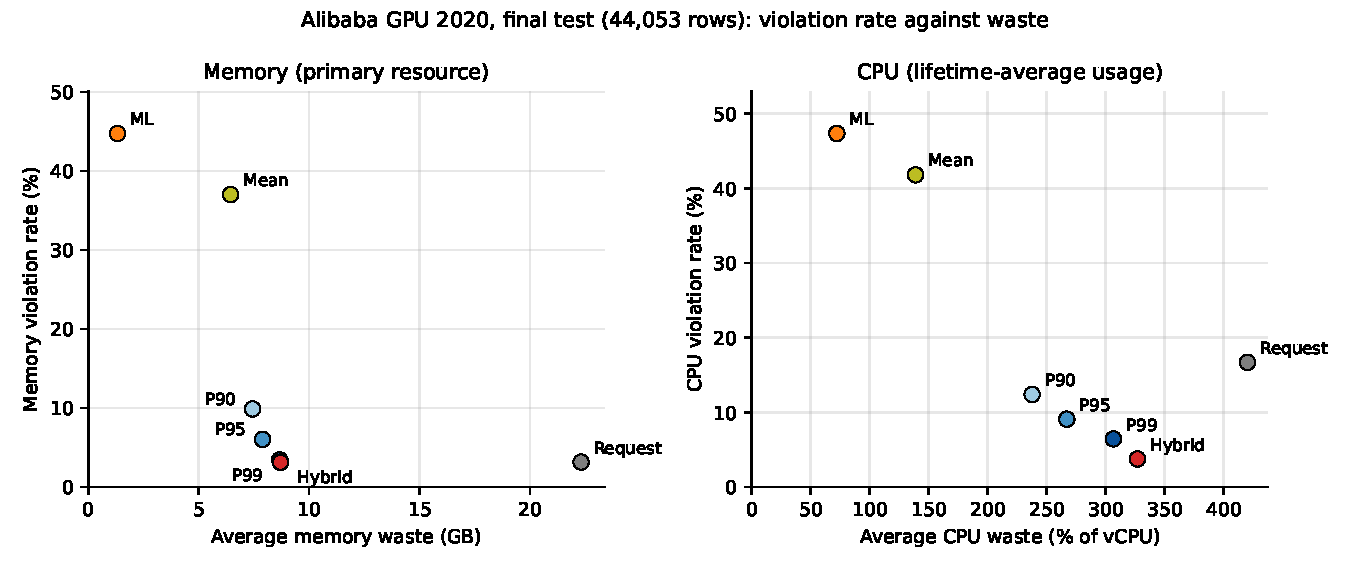
\includegraphics[width=0.92\linewidth]{figures/fig_7_3.pdf}
\caption{Alibaba final test: memory (left) and CPU (right) violation rate versus average waste, 44,053 occurrences}\label{fig:7.3}
\end{figure*}

Overall, the saved final-test results indicate that Hybrid improves reliability relative to its P99 safeguard with only a small increase in average memory waste and a moderate increase in average CPU waste. Although Request achieves a similar memory violation rate, its average memory waste is substantially higher. These findings are limited to the evaluated target definitions, and no combined CPU-or-memory violation rate is reported for Alibaba.

\subsection{Analysis Across Datasets}\label{sec:7.4}

Table~\ref{tab:7.4} summarizes how demand is defined and evaluated on each dataset.

\begin{table*}[!t]
\centering
\footnotesize
\caption{Measurement definitions and evaluation scope for the two evaluation datasets}\label{tab:7.4}
\begin{tabular}{>{\raggedright\arraybackslash}p{0.119\linewidth}>{\raggedright\arraybackslash}p{0.258\linewidth}>{\raggedright\arraybackslash}p{0.254\linewidth}>{\raggedright\arraybackslash}p{0.258\linewidth}}
\hline
\textbf{Dataset} & \textbf{Demand definition and scope} & \textbf{Saved evaluation scope} & \textbf{Interpretation boundary} \\ \hline
Google ClusterData 2019 sample & Full-workload occurrence CPU and memory peaks in normalized units & Baseline, ML, Hybrid; validation and final test & Validation targets cross into the test period \\
Alibaba GPU 2020 & Per-role maximum instance lifetime-average CPU, in percent of one vCPU; maximum instance lifetime memory peak, in GB & Baseline, ML, Hybrid; split-isolated targets and final test & CPU peak demand is unavailable; eligible completed roles with memory telemetry \\
\hline
\end{tabular}
\end{table*}

A key finding across the evaluated datasets is the tradeoff between resource reliability and efficiency. Historical percentile-based recommendations generally reduce resource violations at the cost of increased resource waste, while Hybrid combines ML predictions with historical safeguards to balance these objectives. However, violation rates cannot be directly compared across datasets because their resource targets, measurement units, aggregation methods, filtering criteria, and Hybrid safeguards differ.

Three findings nevertheless hold on both datasets. First, Hybrid had fewer violations than its own safeguard at almost the same waste: on Google, 12.36\% any-resource violations compared with 17.37\% for P95, and on Alibaba, 3.77\% and 3.15\% CPU and memory violations compared with 6.45\% and 3.44\% for P99. Second, ML alone had the lowest waste but under-provisioned about one occurrence in three on Google and almost one in two on Alibaba, so accuracy-driven point predictions are not reliable allocations on their own. Third, the value of the original request differs. Google requests were exceeded by 54.47\% of test occurrences, whereas Alibaba memory requests were exceeded by only 3.16\% at about 2.6 times Hybrid's memory waste.

This difference in requests also explains why the history threshold had opposite effects. Raising \texttt{min\_runs} sends more occurrences to the request fallback. On Google validation, P99's any-resource violation rate rose from 21.95\% at \texttt{min\_runs\ =\ 1} to 30.98\% at \texttt{min\_runs\ =\ 10}, because the fallback requests are often too low; on Alibaba validation, P99's memory violation rate fell from 8.74\% to 5.58\%, because the fallback requests are generous. These are validation observations used for selection, not separate experiments.

\subsection{Discussion of Findings}\label{sec:7.5}

The results show that historical baselines provide a useful reference for reliability, while ML alone reduces resource waste at the cost of higher violation rates. Hybrid achieves lower violation rates than its historical safeguard in both primary datasets. This is consistent with its design: by selecting the maximum of the ML prediction and the historical recommendation, Hybrid cannot recommend fewer resources than the safeguard when both are available.

The key consideration is how much additional protection Hybrid provides and how much additional capacity it requires. The results show a favorable tradeoff relative to the selected historical safeguards, although Hybrid does not outperform every alternative across all evaluation metrics.

The effectiveness of resource requests also varies across datasets. In Google, requested resources frequently fall below subsequent workload peaks, while Alibaba's memory requests achieve reliability comparable to Hybrid but produce substantially greater resource waste. These differences suggest that the usefulness of resource requests as a fallback depends on the resource-requesting practices represented in each dataset. Therefore, a single historical threshold or safeguard should not be assumed optimal across different platforms. Additionally, Alibaba's lifetime-average CPU measurements and role-level aggregation prevent direct numerical comparisons with Google's full-workload peak results.

On Google, 104 of the 329 validation occurrences have next-occurrence targets that start in the test period, because targets were assigned before the chronological split. Restricting validation to the 225 occurrences whose targets remain within it leaves the selected baseline unchanged, with P99's any-resource violation rate moving from 21.95\% to 18.30\% and Hybrid's from 17.93\% to 17.78\%.

Generalizability is further limited by the relatively small Google test population and its sampled trace. The Alibaba evaluation excludes unsuccessful or incompletely observed roles and primarily represents single-instance roles, limiting conclusions about broader distributed workloads, although the multi-instance sensitivity check in Section~\ref{sec:7.3.2} shows the same ordering of Hybrid and P99. Furthermore, the available evidence does not include confidence intervals, repeated-seed experiments, or online deployment measurements. Therefore, the results do not establish statistical superiority, production-level performance improvements, or realized financial savings.
